%% December 2007 
\documentclass[11pt,article]{memoir}     
% Script-based version control (vc package)
\input{vc}

\usepackage{graphicx}
\usepackage{memoir-article-styles}
\usepackage{mysects}
\usepackage{natbib} 
%\usepackage{fancyhdr,fancyvrb}
\usepackage{fontspec}
\usepackage{xunicode}
\usepackage{listings}
\usepackage{listings-sweave-xelatex}
\usepackage[svgnames]{xcolor}
\usepackage{soul}
\sethlcolor{LightGoldenrodYellow}

%\usepackage{xcolor}
%\usepackage{colortbl}
%\usepackage{longtable}

% %\usepackage{sabon}
% \input epsf 

\bibliographystyle{asr}

%\usepackage{/Library/Frameworks/R.framework/Resources/share/texmf/Sweave}

\usepackage[dvipdfm,colorlinks=true,urlcolor=FireBrick,linkcolor=FireBrick,bookmarks=false,citecolor=Black]{hyperref}

\begin{document}
%\chapterstyle{hangnum}
\chapterstyle{article-2} 
\pagestyle{kjh}

\setromanfont[Mapping=tex-text,Numbers=OldStyle]{Minion Pro} 
\setsansfont[Mapping=tex-text]{Myriad Pro} 
% \setmonofont[Mapping=tex-text,Scale=0.7]{Lucida Sans Typewriter} 
%\setmonofont[Mapping=tex-text,Scale=0.7]{Bitstream Vera Sans Mono} 
\setmonofont[Mapping=tex-text,Scale=0.9]{Inconsolata} 

%\frontmatter
\title{\bigskip Choosing Your Workflow Applications}

\author{Kieran Healy}
\date{Sociology Department, Duke University \\ {\scriptsize{\texttt{\href{mailto:kjhealy@soc.duke.edu}{kjhealy@soc.duke.edu}}}}} 


\published{{\scriptsize The most recent version of this document is at} {\scriptsize  \texttt{\href{http://www.kieranhealy.org/files/misc/workflow-apps.pdf}{http://www.kieranhealy.org/files/misc/workflow-apps.pdf}}}}

\maketitle

% \newpage 
%  
% \tableofcontents*            

%\pagestyle{fancy}
%\lhead{}
%\rhead{\footnotesize Choosing Your Workflow Applications \ \thepage}
%\cfoot{}

%\mainmatter
% Include version information in footer. 
\thispagestyle{kjhgit}
 
\begin{abstract}
	As a beginning graduate student in the social sciences, what sort of software should you use to do your work? More importantly, what principles should guide your choice of software? This article offers some answers. The short version is: write using a good text editor (there are several to choose from); analyze data with R or Stata; and minimize errors by keeping your stuff in a simple format (plain text is best), documenting it properly (maybe in a version control system), and back it up sensibly. Don't get bogged down by the gadgets, utilities or other accoutrements: they are there to help you get your work done, but often  waste your time by being beguilingly fun to tweak, update and generally futz with.  
\end{abstract}

\chapter{Introduction} % (fold)
\label{sec:introduction}
You can do productive, maintainable and reproducible work with all kinds of different software set-ups. This is the main reason I don't go around encouraging everyone to convert to the group of applications I myself use. (My rule is that I don't try to persuade anyone to switch if I can't commit to offering them technical support during and after their move.) This discussion is not geared toward convincing you there is One True Way to do your work. I do think, however, that if you're in the early phase of your career as a graduate student in, say, Sociology, or Economics, or Political Science, you should give some thought to how you're going to organize and manage your work.\footnote{This may also be true if you are about to move from being a graduate student to starting as a faculty member, though perhaps the rationale is less compelling given the costs.} This is so for two reasons. First, the transition to graduate school is a good time to make a change in your software platform. Early on, there's less inertia and cost associated with switching things around than there will be later. Second, in the social sciences, text and data management skills are usually not taught to students explicitly. This means that you may end up adopting the practices of your advisor or mentor, continue to use what you are taught in your methods classes, or just copy whatever your peers are using. Following any one of these paths may by chance lead you to an arrangement that you will be happy with. But not all solutions are equally useful or powerful, and you can find yourself locked-in to a less-than-ideal setup quite quickly.

Although I shall describe some specific applications in what follows, in the end it's not really about the gadgets or utilities. It is an obvious but easily-ignored truth that the Zen of Organization is Not to be Found in Fancy Software. Nor shall the True Path of Getting Things Done be revealed to you by way of the purchase of a Nice \href{http://www.moleskineus.com/}{Moleskine Notebook}. Instead, it lies within. For instance, my wife is an academic, too --- a philosopher. Unlike me, she is very well-organized and highly productive. Her task-management system consists of a calendar and some bits of scrap paper with to-do lists scrawled on them. Her work environment is comprised of Microsoft Word, email and a drawer full of candy. No context-dependent Getting-Things-Done system, no bibliographic software, no revision control, nothing. Her super-secret trick is that, when she has a project, she thinks about what needs to be done, writes down a list of tasks on a piece of paper, and then --- and this is the tricky part, which if you're like me you may find hard to follow --- \emph{actually completes these tasks one by one in a systematic fashion}, beginning right away. I know. I didn't understand that last bit, either. Sad to say, only when you have grasped this point will you be able to snatch this list of stuff to do today from her hand, grasshopper. 

For any kind of formal data analysis that leads to a scholarly paper, however you do it, there are basic principles that you will want to adhere to. A key one, for example, is never do anything in a way that doesn't leave a record of your actions. Instead of doing a bit of work and then just keeping the table of results or nice graphic that you produce, always write what you did down as a piece of code or an explicit procedure instead. (You should also document it more fully as you go.) That way, you leave the beginnings of an audit trail. Then when you inevitably return to this table or figure six months down the line, your future self will have been saved hours spent wondering what the hell it was you thought you were doing. A second principle is that a file or folder should always be able to tell you what it is --- i.e., you will need some method for organizing and documenting papers, code, field notes, datasets, output files or whatever it is you're working with. A third principle is that repetitive and error-prone processes should be automated as much as possible. This makes it easier to check for mistakes. Rather than copying and pasting code over and over to do basically the same thing to different parts of your data, write a general function that can be called whenever it's needed. Instead of tediously retyping and reformatting the bibliography for each of your papers as you send it out to a journal, get hold of some software that can manage this for you automatically.

There are many ways of implementing these principles. I present some of them here. You could use Microsoft Word, Endnote and SPSS. Or Textpad and Stata. Or a pile of legal pads, a calculator, a pair of scissors and a box of file folders. It's the principles that matter. But software applications are not all created equal, and some make it easier than others to do the Right Thing. For instance, it is \emph{possible} to produce well-structured, easily-maintainable documents using Microsoft Word. But you have to use its styling and outlining features strictly and responsibly, and most people don't bother. You can maintain reproducible analyses in SPSS, but the application isn't set up to do this automatically or efficiently, nor does its design encourage good habits. So, it is probably a good idea to invest some time learning about the alternatives. Many of them are free to use or try out, and you are at a point in your career where you can afford to play with different setups without too much trouble.
% section introduction (end)   

\chapter{Choice of Platform}

What operating system should you use? The leading candidates are Microsoft Windows, Apple's Mac OS X, and some distribution of Linux. Five or six years ago the conventional wisdom about each of these products was something like this:  
                                                                                      
\begin{itemize}
	\item Windows dominates the market. It is installed by default on most computers. It is not very stable, or secure. When running it you will have to deal with all manner of viruses and malware. It has a very large array of software available for it, especially some relatively esoteric stuff that you can't find anywhere else. It's ugly and badly designed. 
	\item Apple Mac OS X runs only on Apple hardware, which is more expensive than comparable PCs. It is relatively stable and secure. Viruses and malware are not a problem. Underneath the hood it is a version of Unix, so you can run almost all available Unix software, though this may entail some configuration headaches. Most of the software you want is probably available, but there are some exceptions. It's possible to run Windows software on a Mac but it's a real pain, because the underlying hardware architecture is different from PCs. Macs are better designed in almost all respects than almost all PCs, and are easier to use. Specialized software for academics in the social sciences may not be available for the Mac. 
	\item Linux distributions are free and under active development. They are becoming easier to install and configure, but can still be a pain to manage even for quite sophisticated users, assuming you have other things to do. Linux is stable and secure. It is a relative of Unix, so you can run almost all available Unix software. The system-level design is better than Windows. The interface is highly configurable but not nearly as polished as OS X. If you really have to run Windows software some emulation is possible but it's probably better just to have both operating systems installed on your computer. 
\end{itemize}

Today, much of this has changed. Each of the main platforms has gone some of the way --- in some cases a long way --- toward remedying its main defects. I would characterize the changes this way: 

\begin{itemize}
	\item Windows dominates the market. Its most widely-available version, Windows XP, is stable and relatively secure. Because of its market dominance, far more viruses and malware target Windows than any other OS. Design and usability problems have been somewhat ameliorated. The launch of Windows Vista has not been terribly successful, though it's problems do not seem to be ones related to security.

	\item Mac OS X runs only on Apple hardware, but Apple has moved all of its computers over to Intel chipsets. This has two consequences for those considering a move to Mac OS X. First, one can now make direct hardware and price comparisons between Apple computers and PC alternatives (such as Dells, Lenovos, etc). In general, the more similarly kitted-out a PC is to an Apple machine, the more the price difference between the two goes away.\footnote{Such a comparison should still take account of remaining differences in hardware design, and of course the OS itself.} However, Apple does not compete at all price-points in the market, so it will always be possible to configure a cheaper PC (with fewer features) than Apple sells. For the same reason, it is also easier to find a PC configuration precisely tailored to any particular set of specific preferences (e.g., with a better display but without some other feature or other) than may be available from Apple. 
	
	Second, because Apple now runs Intel-based hardware, installing and running Windows is easy, and even catered to by Mac OS. Beyond installing OS X and Windows side-by-side, third-party software is available (for about \$80 from \href{http://www.vmware.com/products/fusion/}{VMWare} or \href{http://www.parallels.com/}{Parallels}) that allows you to run Windows (or Linux) seamlessly within OS X. 
	\item Linux is stable, secure and free. It has improved substantially in its ease of installation and use. User-oriented distributions such as \href{http://www.ubuntu.com/}{Ubuntu} are much better-integrated and well-organized than in the past. The user environment is much friendlier. In particular, installing, upgrading and updating software --- a key point of frustration and time-wasting in older Linux distributions --- is also much better than it used to be. It remains true that Linux users are more likely to be forced at some point to learn more than they might want to about the guts of their operating system.
	
\end{itemize}

These days, I use Mac OS X. But the other two options are also perfectly viable alternatives. Rather than try to convince you to plump for one option or another, the next section describes some applications that run on all of these operating systems.\footnote{I will say that one advantage of buying Mac hardware is that it allows you, should you wish, to install and run all three platforms side-by-side.} 


\chapter{A Sample Set of Applications} 

The dissertation and articles you write will generally consist of the main text, the results of data analysis (perhaps presented in tables or figures) and the scholarly apparatus of notes and references. Thus, as you  put a paper or an entire dissertation together you will want to be able to easily \textbf{edit text}, \textbf{analyze data} and \textbf{minimize error}. The following applications are designed to let you do this easily. They fit together well (by design) and are all freely available for Windows, Linux and Mac OS X. They are not perfect by any means, and indeed some of them are kind of a pain in the ass to learn. (I'll discuss some alternatives later.) But they are designed to help with many of the specialized tasks associated with analyzing data and writing scholarly papers.                                                      

\section{Edit Text}
If you are going to be doing quantitative analysis of any kind then you should learn to use a good text editor. The same is true, I'd argue, for any highly structured document subject to a lot of revision, such as a scholarly paper. Unlike applications such as Microsoft Word, text editors generally don't make a big effort to make what you write look like as though it is being written on a printed page. Instead, they focus on manipulating text efficiently. If you are writing code to run in a statistics program, at a minimum a good editor will highlight the syntax of your code in a way that makes it more readable. Typically it will also passively signal to you when you've done something wrong (like forget a closing brace or semicolon or quotation mark), \href{http://en.wiktionary.org/wiki/automagical}{automagically} indent or tidy up your code in an intelligent way. If you are writing a scholarly paper or a dissertation, a good text editor can make it easier to maintain control over the structure of your document, and help ensure that cross-references and other paraphernalia are correct. And just as the actual numbers are crunched by your stats program --- not your text editor --- the typesetting of your paper is handled by a specialized application, too.

\smallskip

\textbf{Emacs} is a text editor, in the same way the blue whale is a mammal. Emacs is very powerful, and can become almost a complete working environment in itself, should you so wish. (I don't really recommend it.) Combining Emacs with some other applications and add-ons (described below) allows you to manage writing and data-analysis effectively. The \href{http://www.gnu.org/software/emacs/}{Emacs Homepage} has links to Windows and Linux versions. The best version on the Mac is \href{http://aquamacs.org/}{Aquamacs}, as it makes an effort to integrate Emacs with the Mac OS. For Windows users who would like to use Emacs, John Fox has a
\href{http://socserv.mcmaster.ca/jfox/Books/Companion/ESS/}{very useful page}
containing a customized XEmacs distribution and instructions for how to install and
configure it for quantitative analysis with R (about which more below).

While very powerful and flexible, Emacs is not particularly easy to learn. Because it evolved in a much  earlier era of computing (before decent graphics displays, for instance), it doesn't share many of the conventions of modern applications. There are numerous good alternatives, and I discuss some of them in subsequent sections. I recommend it here because, despite its shortcomings, it is very, very good at managing the typesetting and statistics applications I'm about to discuss.

\smallskip

\textbf{LaTeX} is a freely-available, professional-quality typesetting system. It takes text marked up with annotations indicating the desired structure and formatting (where the sections and subsections are, for example, or whether text should be \textbf{in bold face} or \emph{emphasized}) and processes it into a properly typeset document. If you have ever edited the HTML of a web page, you'll know the general idea of a markup language. If you haven't, the easiest way to understand what I mean is to look at a segment of LaTeX markup. An example is shown in Figure \ref{fig:latex}. This document is written in LaTeX markup. You can get started with TeX and LaTeX for Mac OS X \href{http://tug.org/mactex/}{from this page}. On Windows, \href{http://www.miktex.org/}{MiKTeX} is a widely-used version of TeX. The \href{http://www.tug.org/pracjourn/}{PracTeX Journal} is an excellent source of information on how to do work using LaTeX. 

\begin{figure}
%  \begin{Verbatim}[frame=single,fontsize=\footnotesize]
\begin{lstlisting}[style=sweave-top]
\end{lstlisting}
\begin{lstlisting}[language={[latex]tex},numbers=none,style=sweave-tex]
\section{Edit Text}

\textbf{LaTeX} is a freely-available, professional-quality typesetting
  system. It takes text marked up with annotations indicating the desired
  structure and formatting (where the sections and subsections are, for example, 
  or whether text should be \textbf{in bold face} or \emph{emphasized}) and 
  processes it into a properly typeset document. If you have ever edited the 
  HTML of a web page, you'll know the general idea of a markup language. If you 
  haven't, the easiest way to understand what I mean is to look at a segment 
  of LaTeX markup. An example is shown in Figure \ref{fig:latex}.

 
\end{lstlisting}
\begin{lstlisting}[style=sweave-bottom]
\end{lstlisting}
\caption{The LaTeX source for part of a previous version of this document.}
\label{fig:latex}
\end{figure}

\smallskip

\textbf{Other LaTeX Tools}. LaTeX works best with some tools that help you take full advantage of it with a minimum of fuss. You can manage bibliographical references in LaTeX documents using \textbf{BibTeX}. It does the same job as \href{http://www.endnote.com/}{\textbf{Endnote}}, the commercial plug-in for managing references in Microsoft Word. BibTeX comes with any standard LaTeX installation. Whatever text editor or word processor you use, you should strongly consider some kind of reference-manager software for your bibliographies. It saves a tremendous amount of time because you can easily switch between bibliography formats, and you don't have to worry whether every item referenced in your dissertation or paper is contained in the bibliography.\footnote{If you plan to use BibTeX to manage your references, be sure to look into \href{http://www.ctan.org/tex-archive/help/Catalogue/entries/biblatex.html}{BibLaTeX}, a promising new package from Philipp Lehman designed to overcome some of BibTeX's limitations. BibLaTeX is not yet stable, but is being actively developed.} \textbf{\href{http://www.gnu.org/software/auctex/}{AUCTeX}} and \textbf{RefTeX} are typically bundled along with Emacs. These packages allow Emacs to understand the ins and outs of typesetting LaTeX documents. AUCTeX color-codes the marked-up text to make it easier to read, and it has keyboard shortcuts for producing all the necessary formatting commands for LaTeX. RefTeX helps you outline documents more easily, and also manages references to Figures, Tables and bibliographic citations in the text. Both these packages could also be listed under the ``Minimize Error'' section below, because they automagically ensure that, e.g., your references and bibliography will be complete and consistent.\footnote{A note about fonts and LaTeX. It used to be that getting LaTeX to use anything but a relatively small set of fonts was a very tedious business. This is no longer the case. The \href{http://scripts.sil.org/cms/scripts/page.php?site_id=nrsi&id=xetex}{XeTeX} engine makes it trivially easy to use any Postrcript, TrueType or OpenType font installed on your system. XeTeX was originally developed for use on the Mac, but is available now for Linux and Windows as well.} 

More information on Emacs and LaTeX is readily available via Google, and there are several excellent books available to help you get started. \citet{kopka03:_guide_latex} and \citet{mittlebach04:_latex_compan} are good resources for learning LaTeX. The latter comes with a CD containing a complete LaTeX installation for Linux and Windows. For further argument about the advantages of text-editors over word processors see Allin Cottrell's polemic, ``\href{http://www.ecn.wfu.edu/~cottrell/wp.html}{Word Processors: Stupid and Inefficient}.''
     
\section{Analyze Data and Present Results} 
You will probably be doing some --- perhaps a great deal --- of quantitative data analysis. \textbf{R} is an environment for statistical computing. It's exceptionally well-supported, continually improving, and has a very active user community who have produced many add-on packages. R has the ability to produce sophisticated and high-quality statistical graphics. The documentation that comes with the software is complete, if somewhat terse, but there are a large number of excellent reference and teaching texts that illustrate its use. These include \citet{dalgaard02:_introd_statis_r}, \citet{venables02:_moder_applied_statis_s_plus}, \citet{maindonald03:_data_analy_graph_using_r}, \citet{fox02:_r_s_plus_compan_applied_regres}, \citet{frank01:_regres_model_strat}, and 
\citet{gelmanhill07:data_analysis}. Although it is a command-line tool at its core, it has a good graphical interface as well. You can download it from \href{http://www.r-project.org/}{The R Project Homepage}.     

R can be used directly within Emacs by way of a package called \textbf{ESS}
(for ``Emacs Speaks Statistics''). As shown in Figure~\ref{fig:ess}, it allows you to work with your code in one Emacs frame and a live R session in another right beside it. Because everything is inside Emacs, it is easy to do things like send a chunk of your code over to R using a keystroke. This is a very efficient way of doing interactive data analysis while building up code you can use again in future.  

\begin{figure}[h]
	\centering
		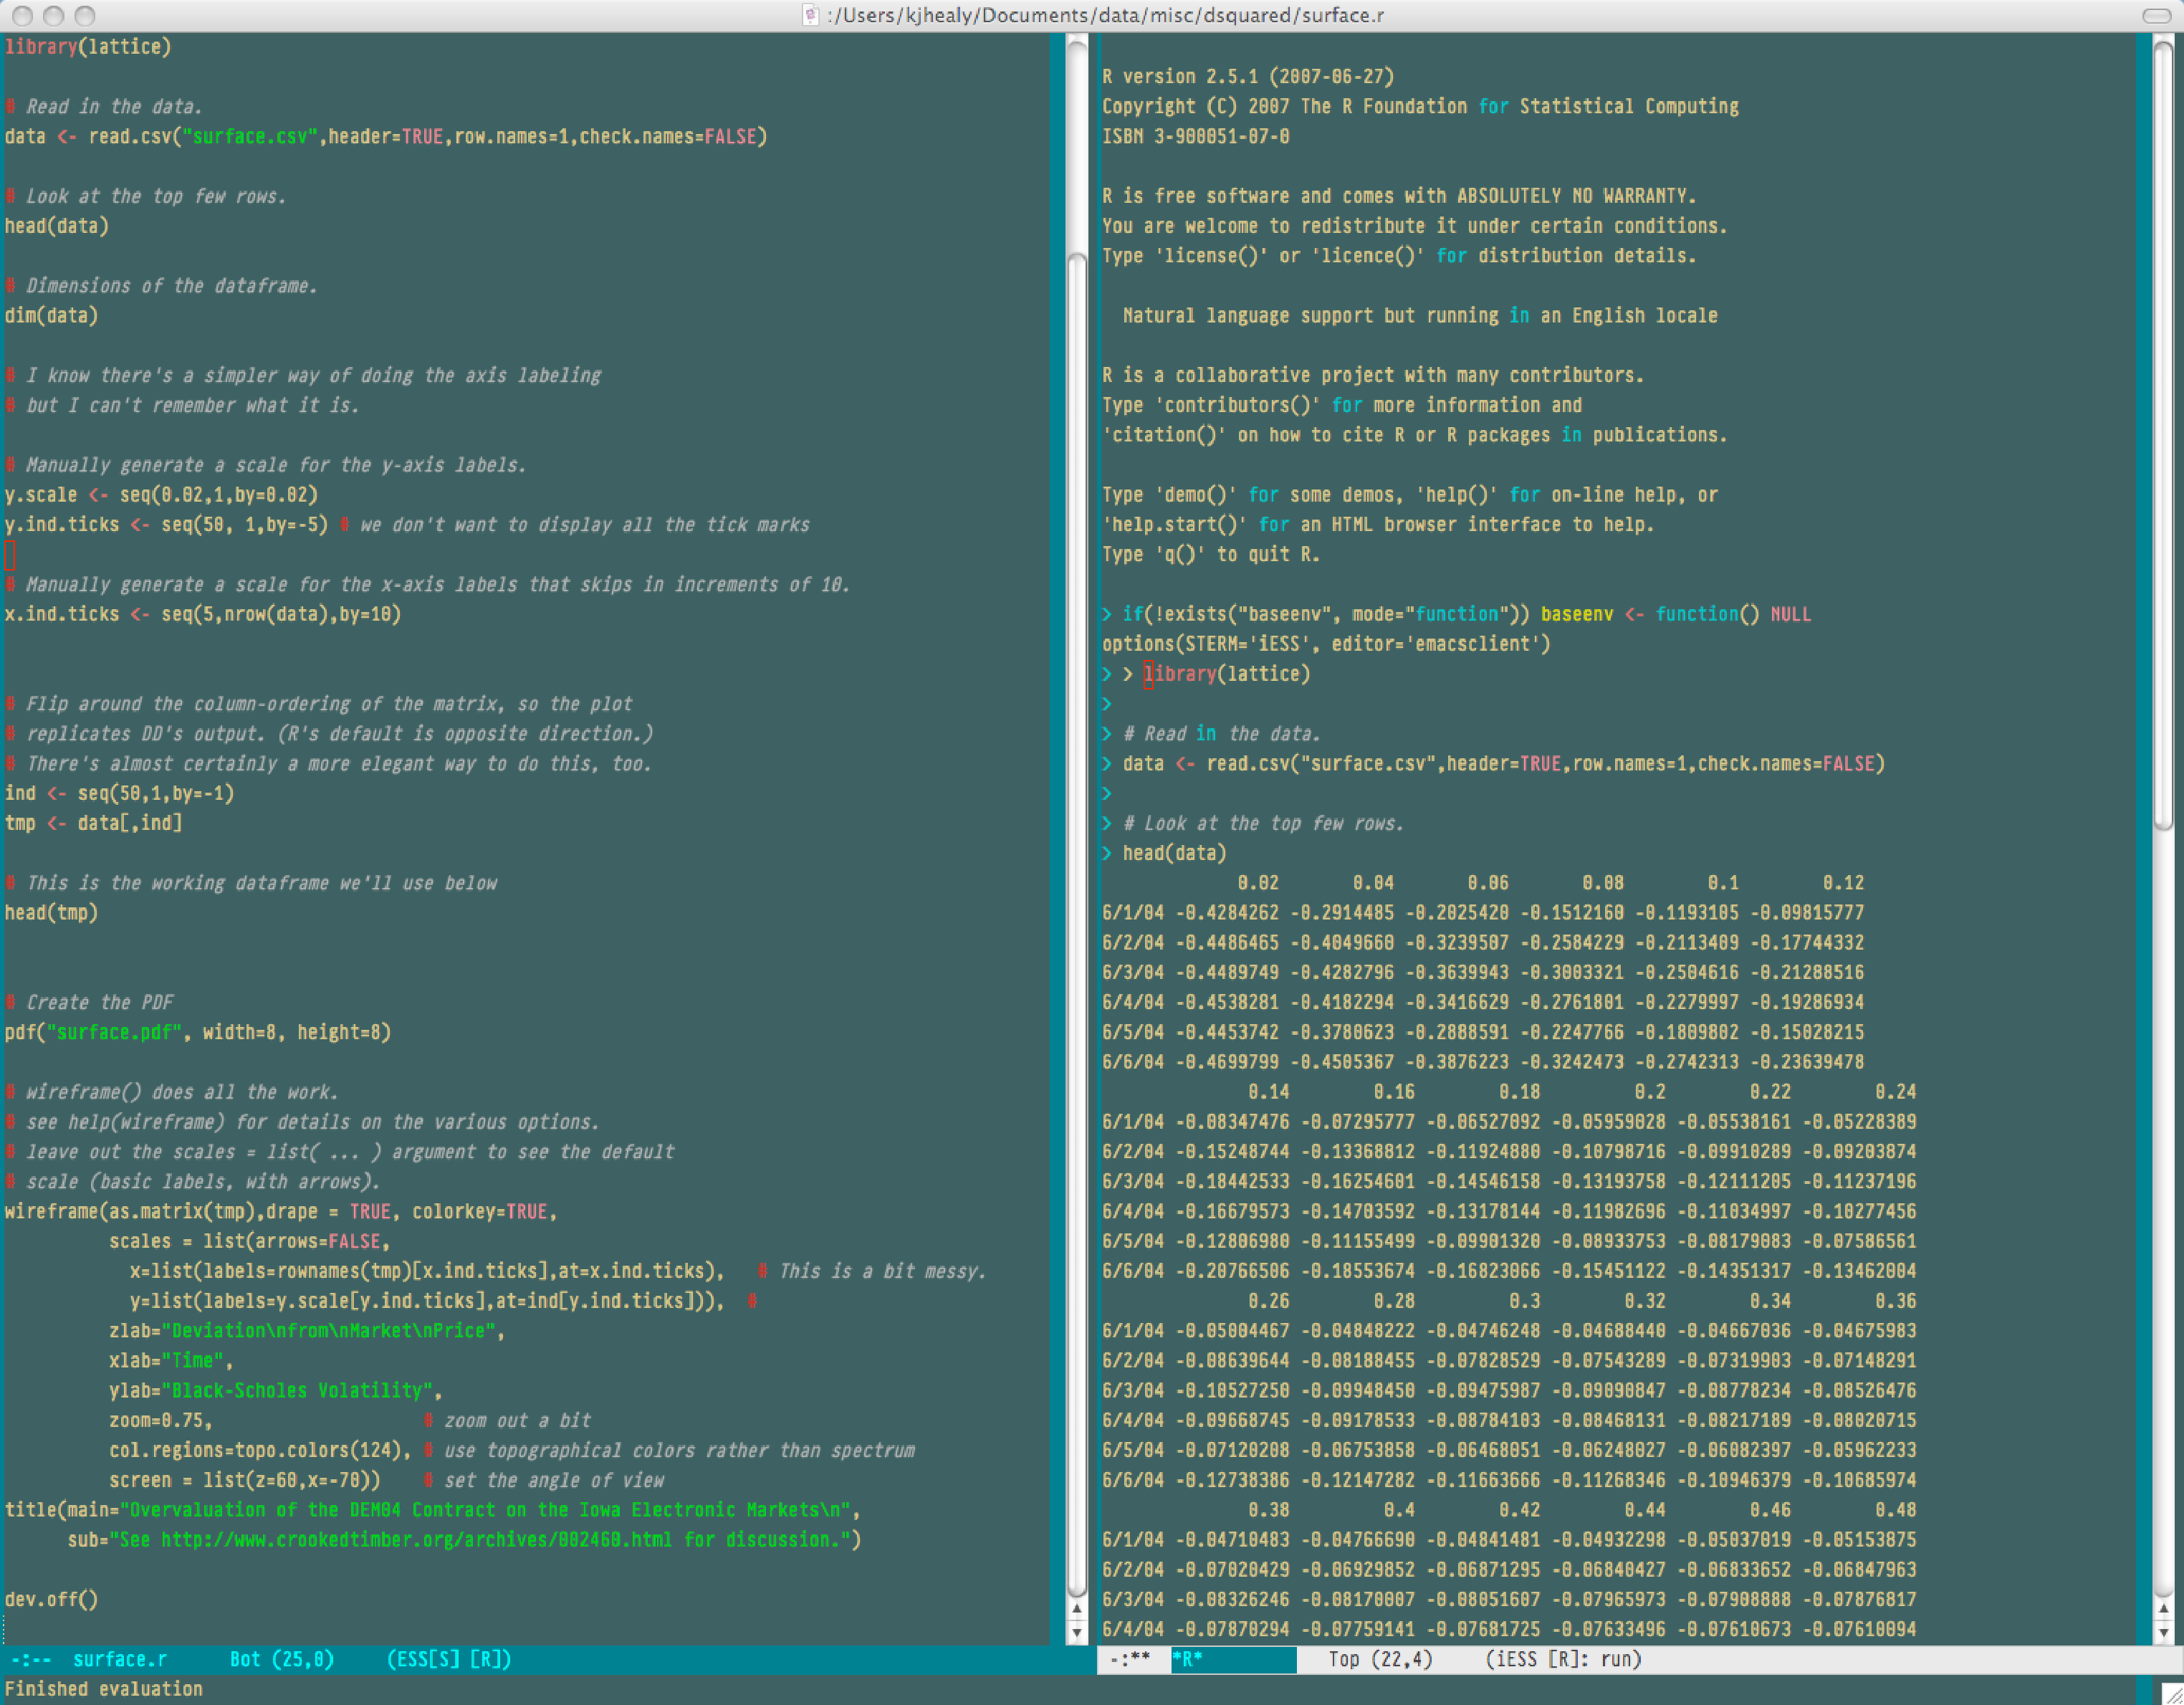
\includegraphics[scale=0.25]{figures/EmacsESS2}
	\caption{An R session running inside Emacs using ESS. The R code file is on the left, and R itself is running on the right.}
	\label{fig:ess}
\end{figure}
                           
\section{Minimize Error}  
A significant source of error in data analysis is the gap between the procedure used to produce a figure or table in a paper and the subsequent use of that output later. In the ordinary way of doing things, you have the code for your data analysis in one file, the output it produces in another, and the text of your paper in a third file. You do the analysis, collect the output and copy the relevant results into your paper (often manually reformatting them on the way). Each of these transitions introduces the opportunity for error. It also makes it harder for you (let alone anyone else) to reproduce your work later, as the output becomes detached from the actions that produced it. Almost everyone who has written a quantitative paper has been confronted with the problem of reading an old draft containing results or figures that need to be revisited, but you can't quite remember how they were produced. 

\smallskip

\textbf{Sweave} is a \emph{literate programming} framework designed to solve this kind of problem by integrating the text describing your data analysis with the R code that does the analysis. This allows you to write self-documenting code and makes your work easy (for you and others) to reproduce. With Sweave, you just have one file for both the data analysis and the writeup, and figures are created on the fly. You write the text of your paper (or, more often, your report of a data analysis) as normal. Whenever you want to run a model, produce a table or display a figure, rather than paste in the results of your work from elsewhere, you write a ``chunk'' of R code that will produce the output you want. Each code-chunk is distinquished from the regular text by a special delimiter at its beginning and end. A small sample is shown in Figure \ref{fig:codechunk}. The code chunk begins with the line \lstinline!<<load-data, echo=true>>=!. The character sequence \lstinline!<<>>=! is the marker for the beginning of a chunk: \lstinline!load-data! is just a label for the chunk and \lstinline!echo=true! is an option. The end of each chunk is marked by the \lstinline!@! symbol.


\begin{figure}
\begin{lstlisting}[style=sweave-top]

\end{lstlisting} 
\begin{lstlisting}[language={[latex]tex},numbers=none,style=sweave-tex]   
\section{Some exploratory analysis}
\label{sec:exploratory}
In this section we do some exploratory analysis of the data. We begin by
reading in the data file:
\end{lstlisting}
\begin{lstlisting}[language=R,numbers=none,style=sweave-r] 
<<load-data, echo=true>>=
# load the data. 
my.data <- read.csv("data/sampledata.csv",header=TRUE)

# OLS model
out <- lm(y ~ x1 + x2,data=my.data)

summary(out)

# ... More R code would follow until the end delimiter:

@ 
\end{lstlisting}
\begin{lstlisting}[language={[latex]tex},numbers=none,style=sweave-tex] 
% now we are back to normal latex 
This concludes the exploratory analysis. 
\end{lstlisting} 
\begin{lstlisting}[style=sweave-bottom]

\end{lstlisting}
  \caption{A chunk of R code in a LaTeX document.}
\label{fig:codechunk}
\end{figure}

When you're ready, you ``weave'' the file: you feed it to R, which processes the code chunks, and spits out a finished version where the code chunks have been replaced by their output. This is now a well-formed LaTeX file that you can then turn into a PDF document in the normal way. It's pretty straightforward in practice. I've included an example at the end of this document that shows how it works.

The strength of this approach is that is makes it much easier to document your work properly (and elegantly) and it makes reproducing a data analysis much easier as well. If you need to do multiple but identical (or very similar) analyses of different bits of data, Sweave can make generating consistent and reliable reports much easier.

A weakness of the Sweave model is that when you make changes, you have to reprocess the all of the code to reproduce the final LaTeX file. If your analysis is computationally intensive this can take up time. There are \emph{ad hoc} ways around this, such as designing one's projects so that they are relatively modular, or selectively processing code chunks. The latter may eventually appear as a  feature in a future version of Sweave. Sweave comes built-in to R. Sweave files can be edited in Emacs, as ESS understands them.

\smallskip

The task of documenting your work at the level of particular pieces of code or edits to paragraphs in individual files can become more involved over time, as projects grow and change. One option is to institute some kind of \textbf{version} \textbf{control} \textbf{system} to allow you to keep a complete record of changes to a file, a folder, or group of folders. This allows you to revisit earlier versions of papers and data analyses without having to keep directories full of files with names like Paper-1.tex, Paper-2.tex, Paper-3-a-i.tex, and so on. Modern version control systems include \href{http://subversion.tigris.org/}{Subversion}, \href{http://www.selenic.com/mercurial/}{Mercurial} and \href{http://git.or.cz/}{Git}. They are powerful tools able to manage large projects spread across multiple users. As such, they require a little time to get comfortable with, mostly because you have to learn some new concepts related to tracking your files. They might seem like overkill for individual users, but they can be used fairly straightforwardly in a basic fashion and they have significant benefits. It can be extremely useful to be able to document changes to a project on the fly, easily test out alternative lines of development by branching a project, and have the ability to revisit any stage of a project's development at will.\footnote{Mercurial and Git are \emph{distributed} revision control systems (DVCSs) which can handle projects with very complex, decentralized organizational forms. Bryan O'Sullivan's \href{http://hgbook.red-bean.com/hgbook.pdf}{\emph{Distributed Version Control with Mercurial}} is a guide to one of the main DVCS tools, but also provides a clear account of how modern version-control systems have developed, together with the main concepts behind them.} If you do not use a formal revision control system, you should nevertheless have some kind of systematic method for keeping track of versions of your files.

Related to version control is the problem of synchronization. I have a laptop and a desktop. I want to keep certain folders in both home directories synchronized. \textbf{Unison} is an efficient command-line synchronization tool that can work locally or use SSH for remote clients. It can also be used for backing up your data. There's a menu-driven, graphical version available as well. It's free. Learn more at \href{http://www.cis.upenn.edu/~bcpierce/unison/}{Unison's homepage}. Other file synchronization tools are available for Mac OS X and Windows, but I haven't used many of them. 

Even if you have no need for a synchronization application, you will need to back up your work regularly. The most useful systems are those that require a minimum amount of work to set up and back up your work automatically to an external (or remote) hard disk without you having to remember to activate them. On newer Macs, Apple's \textbf{Time Machine} software makes this easy. On Linux, you can use \href{http://www.psychocats.net/ubuntu/backup}{rsync} for backups. It is also  worth looking into a secure, offsite backup service like \href{http://mozy.com/}{\textbf{Mozy}}. These services are relatively cheap, and allow you to automatically and securely back up your data. It also means that in the event (unlikely, but not unheard of) that your computer \emph{and} your local backups are stolen or destroyed, you will still have copies of your files.\footnote{I know of someone whose office building was hit by a tornado. She returned to find her files and computer sitting in a foot of water. You never know.}

\section{Pros and Cons}  
Using Emacs, LaTeX and R together has four main advantages. First, these applications are all free. You can try them out without much in the way of expense. Second, they are all open-source projects and are all available for Mac OS X, Linux and Windows. Portability is important, as is the long-term viability of the platform you choose to work with. If you change your computing system, your work can move with you easily. Third, they deliberately implement ``best practices'' in their default configurations. Writing documents in LaTeX encourages you to produce papers with a clear structure, and the output itself is of very high quality aesthetically. Similarly, by default R implements modern statistical methods in a high-quality way that discourages you from thinking about statistics in terms of canned solutions to standard problems. It also produces figures that accord with accepted standards of efficient and effective information design. And fourth, the applications are closely integrated. Everything can work inside Emacs, and all of them talk to or can take advantage of the others. R can output LaTeX tables, for instance, even if you don't use Sweave.

None of these applications is perfect. Some of them have steep learning curves. However, you don't have to start out using all of them at once. (I certainly didn't.) There are a number of ways to try them out in whole or in part. You could try LaTeX first, using any editor. Or you could try Emacs and LaTeX together. You could begin using R and its GUI.\footnote{If you already know Emacs, you should certainly try R using ESS instead of the R GUI, though.} Sweave can be left till last, though I've found it increasingly useful since I've started using it, and wish that all of my old data directories were documented in this format. 

You are not condemned to use these applications forever. LaTeX documents can be converted into other formats. Your text files are directly editable in any other text editor. Statistical code is by nature much less portable, but the openness of R means that it is not likely to become obsolete or inaccessible any time soon.

A disadvantage of these particular applications is that I'm in a minority with respect to other people in my field. This is less and less true in the case of R, but remains so for LaTeX. Most people use Microsoft Word to write papers, and if you're collaborating with people (people you can't boss around, I mean) this can be an issue. Similarly, journals and presses in my field generally don't accept material marked up in LaTeX, though again there are exceptions. Converting files to a format Word understands can be tedious (although it is quite doable).\footnote{If you really want to maximize the portability of your papers or especially your reading notes or memos, consider writing them in a modern lightweight markup format  such as \href{http://en.wikipedia.org/wiki/Markdown}{Markdown} or its close relation, \href{http://fletcherpenney.net/MultiMarkdown}{MultiMarkdown}. Documents written in this format are easy to read in their plain-text form but can be simply and directly converted into HTML, Rich Text, LaTeX, Word, or other formats. TextMate has good support for Markdown and MultiMarkdown, allowing you to do these conversions more or less automatically. Relatedly, John MacFarlane's \href{http://johnmacfarlane.net/pandoc/}{Pandoc} is a tool that can read markdown and (subsets of) reStructuredText, HTML, and LaTeX; and it can write to MarkDown, reStructuredText, HTML, LaTeX, ConTeXt, RTF, DocBook XML, groff man, and S5 HTML slide shows.} I find the day-to-day benefits outweigh these headaches. Your mileage, as they say, may vary.

\begin{figure}[ht]
	\centering
		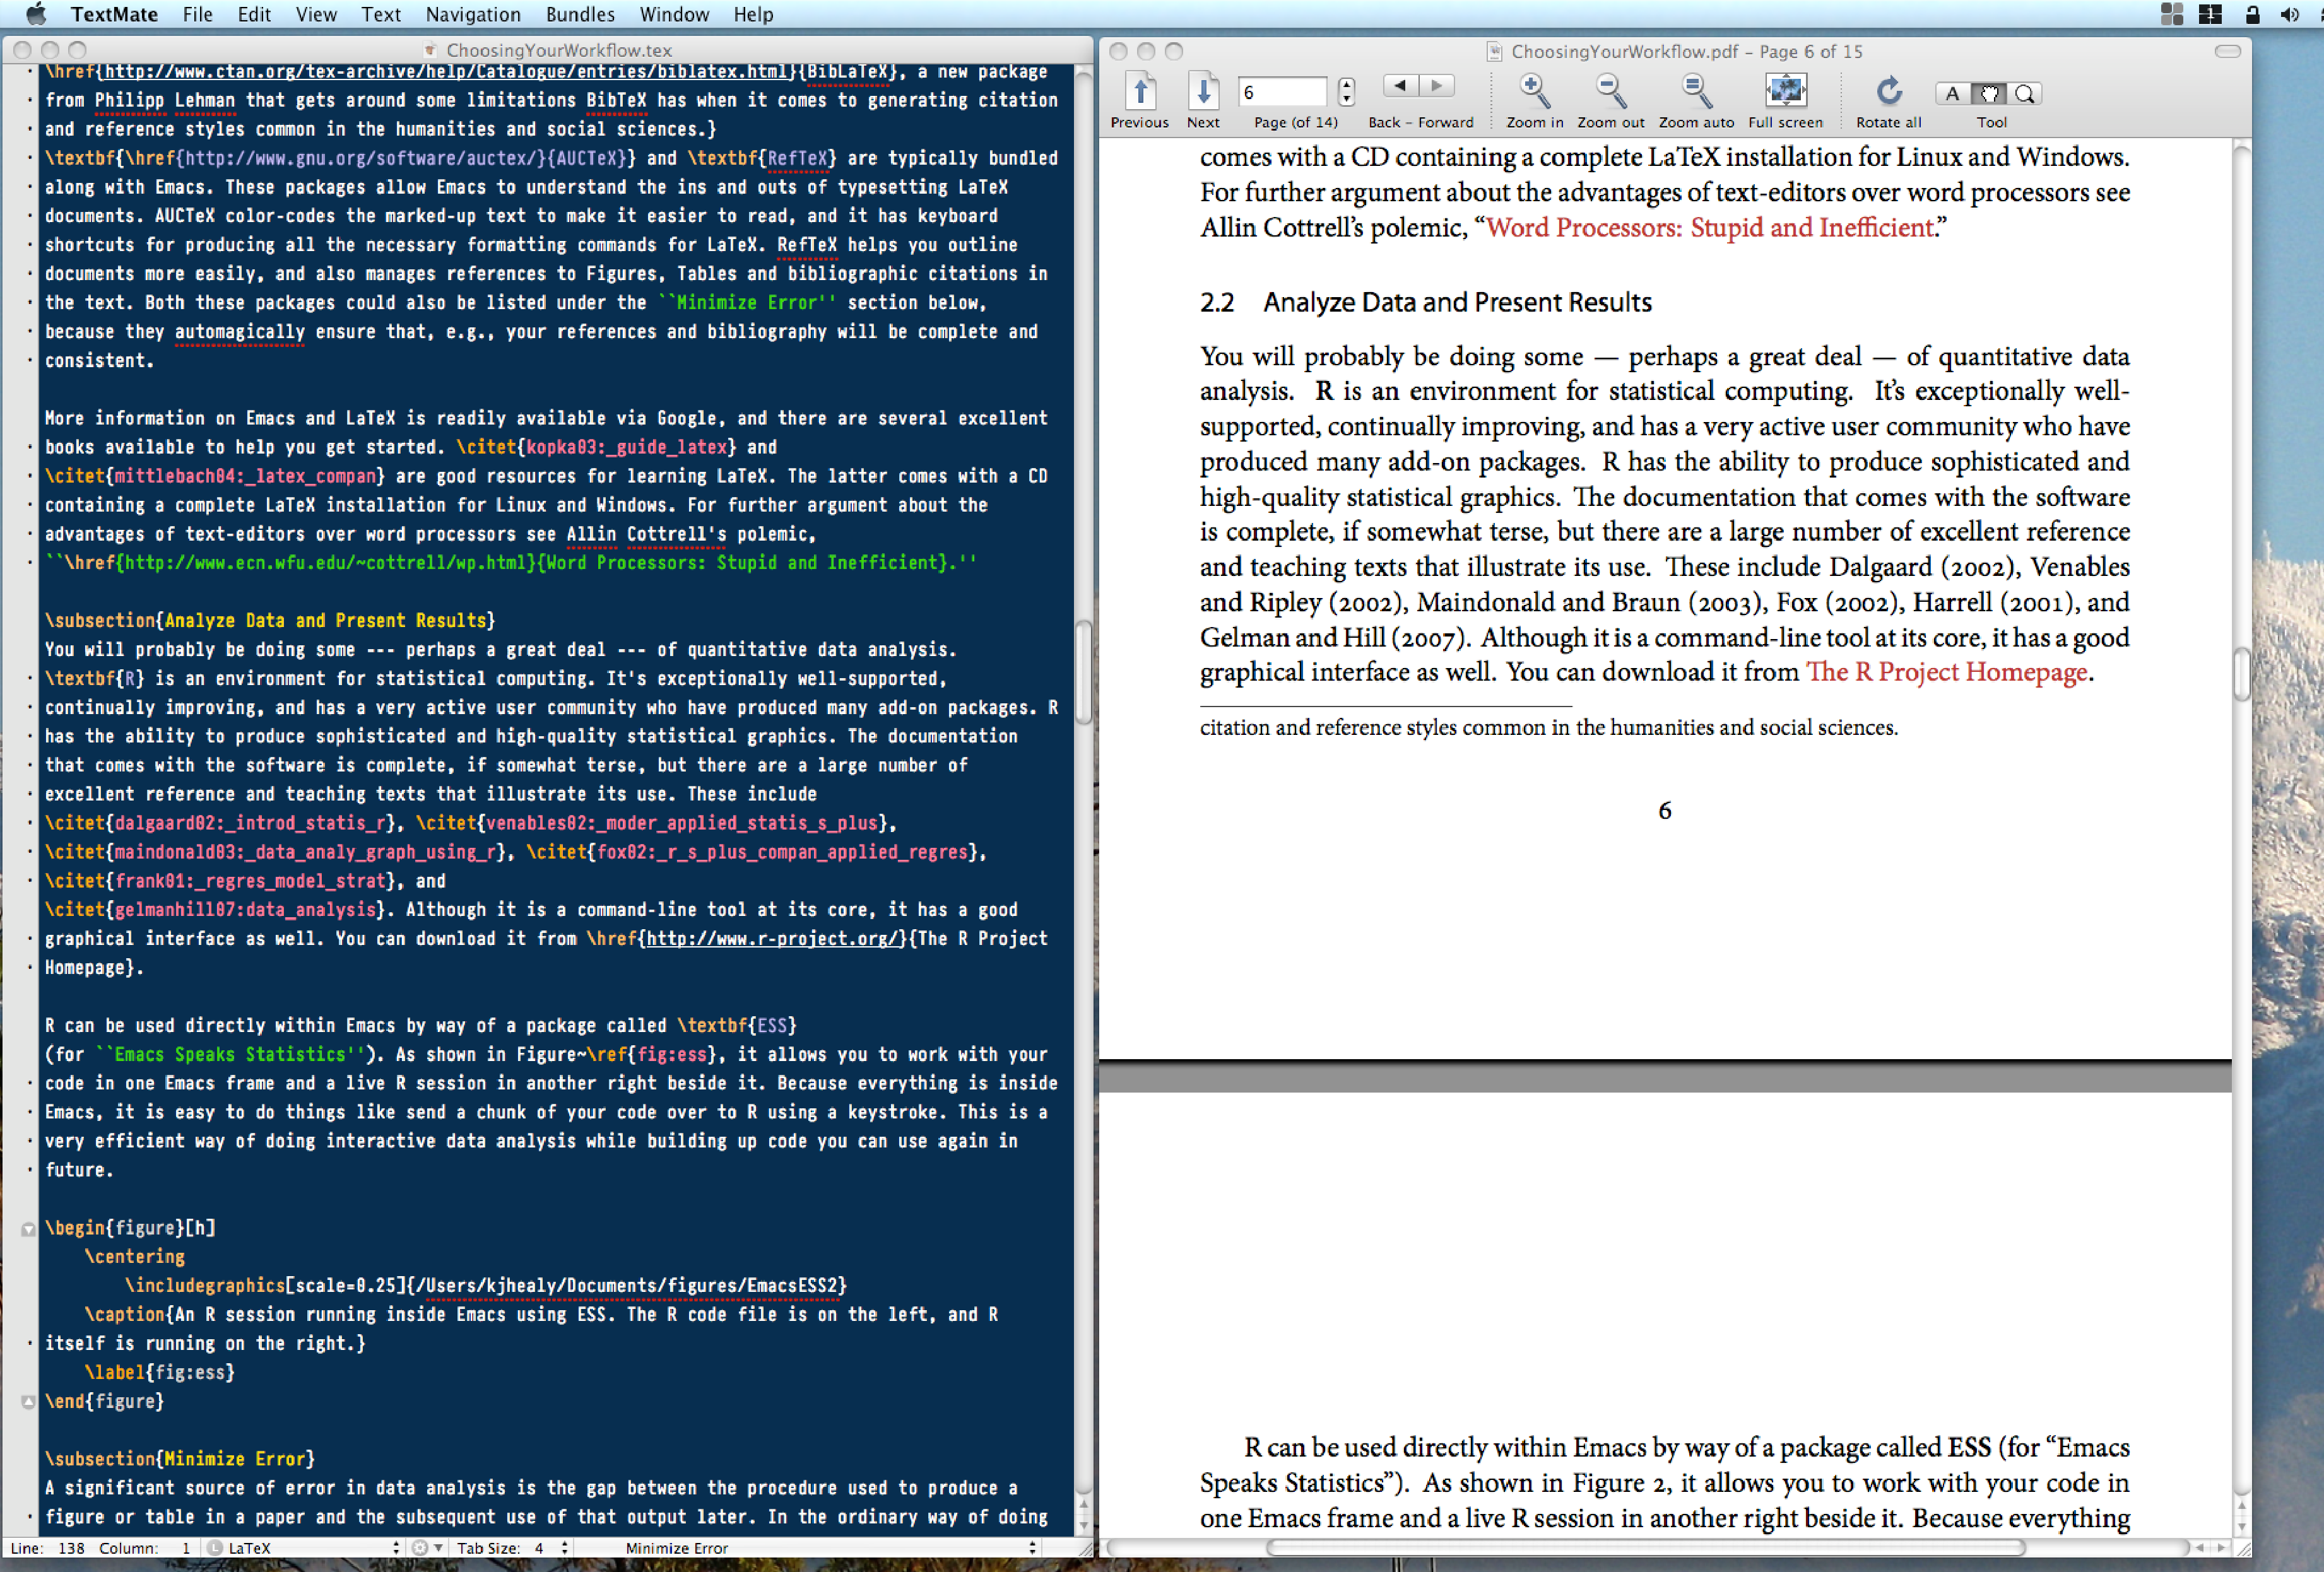
\includegraphics[scale=0.2]{figures/TextMateLaTeX}
	\caption{Editing this document in TextMate (left) with the typeset output on the right. Note how section titles, citations and hyperlinks are represented in the editor and how they appear in the typeset document.}
	\label{fig:label}
\end{figure}

\chapter{Alternative Applications}
There are many other applications you might put at the center of your workflow, depending on one's needs, personal preferences, willingness to pay some money, or desire to work on a specific platform. For \textbf{text editing}, especially, there is a plethora of choices. On the Mac, quality editors  include
\href{http://www.barebones.com/products/bbedit/index.shtml}{BBEdit}, \href{http://smultron.sourceforge.net/}{Smultron} and \href{http://macromates.com/}{TextMate}. I strongly recommend taking a look at TextMate: it's the editor I use for most of my day-to-day work. It has strong support for LaTeX and increasingly good (meaning, ESS-like) support for R. Because it is a modern application written specifically for the Mac it can take advantage of features of OS X that Emacs cannot, and is much better integrated with the rest of your system. It has good support for many of the ancillary applications discussed above, such as version control systems. On Linux, an alternative to Emacs is \href{http://www.eng.hawaii.edu/Tutor/vi.html}{vi} or \href{http://www.vim.org/}{Vim}, but there are many others. For Windows there is \href{http://www.textpad.com/}{Textpad}, \href{http://www.winedt.com/}{WinEdt}, \href{http://www.ultraedit.com/}{UltraEdit}, and \href{http://notepad-plus.sourceforge.net/uk/site.htm}{NotePad++} amongst many others. Most of these applications have strong support for LaTeX and some also have good support for statistics programming.

For statistical analysis in the social sciences, the main alternative to R is \href{http://www.stata.com/}{Stata}. Stata is not free, but like R it is versatile, powerful, extensible and available for all the main computing platforms. It has a large body of user-contributed software. In recent versions its graphics capabilities have improved a great deal. ESS can run Stata inside Emacs in the same way as it can do for R. Other editors can also be made to work with Stata: Jeremy Freese provides an  \href{http://www.jeremyfreese.com/#other%20research}{UltraEdit syntax highlighting file for Stata}. Friedrich Huebler has a \href{http://mysite.verizon.net/huebler/2005/20050310_Stata_editor.html}{guide for integrating Stata with programming editors}. And there is also a \href{http://www.winedt.org/Config/modes/Stata.php}{Stata mode} for WinEdt.


\chapter{A Broader Perspective} 
It would be nice if all you needed to do your work was a bunch of well-written and very useful applications. But of course it's a bit more complicated than that. In order to get to the point where you can write a paper, you need to be organized enough to have collected some data, read the right literature and, most importantly, asked an interesting question. No amount of software is going to solve those problems for you. In fact, too much concern with the details of your setup can hinder your work. The besetting vice of an enthusiasm for productivity-enhancing software is the tendency to waste a lot of your time installing, updating and generally obsessing about your productivity-enhancing software. This is why it helps to bear in mind that it's the principles of workflow management that are really important, and the software is just a means to an end. Even more generally, efficient workflow habits are themselves a means to the end of completing the projects you are really interested in. The process of idea generation and project management can be run efficiently, too, and perhaps even the business of choosing what the projects should be in the first place. But this is not the place --- and I'm not sure I'm the person --- to be giving advice on those kinds of questions.

\appendix

\chapter{An Sweave Example} % (fold)
\label{sec:an_sweave_example}

% appendix an_sweave_example (end)
\label{sec:append-sweave-exampl}
Consider the \texttt{cats} regression example from
\citet{venables02:_moder_applied_statis_s_plus}.\footnote{This example comes
  directly from the \href{http://www.ci.tuwien.ac.at/~leisch/Sweave/}{Sweave documentation}.} The data contains 
measurements of heart and body weight of 144 cats (47 female, 97 male). A
linear regression model of heart weight by bodyweight and sex can be fitted in
R using the command

% \begin{Schunk}
% \footnotesize
% \begin{Sinput}
\begin{lstlisting}[language=R,numbers=none]
> lm1 <- lm(Hwt ~ Bwt * Sex, data = cats)
\end{lstlisting}
% \end{Sinput}
% \end{Schunk}
\normalsize 
Tests for significance of the coefficients are shown in
Table~\ref{tab:coef}, a scatter plot including the regression lines is
shown in Figure~\ref{fig:cats}.

% latex table generated in R 2.0.0 by xtable 1.2-4 package
% Wed Oct 27 17:06:09 2004

\begin{table}[ht]
\footnotesize
\begin{center}
\begin{tabular}{rrrrr}
\hline
 & Estimate & Std. Error & t value & Pr($>$$|$t$|$) \\
\hline
(Intercept) & 2.9813 & 1.8428 & 1.62 & 0.1080 \\
Bwt & 2.6364 & 0.7759 & 3.40 & 0.0009 \\
SexM & $-$4.1654 & 2.0618 & $-$2.02 & 0.0453 \\
Bwt:SexM & 1.6763 & 0.8373 & 2.00 & 0.0472 \\
\hline
\end{tabular}
\caption{\small Linear regression model for cats data.}
\label{tab:coef}
\end{center}
\end{table}
\normalsize 

In this example, the code chunks that produce Table \ref{tab:coef} and Figure
\ref{fig:cats} are replaced by their output when the final document is produced. 

\begin{figure}[h!]
  \centering
\setkeys{Gin}{width=0.55\textwidth} 
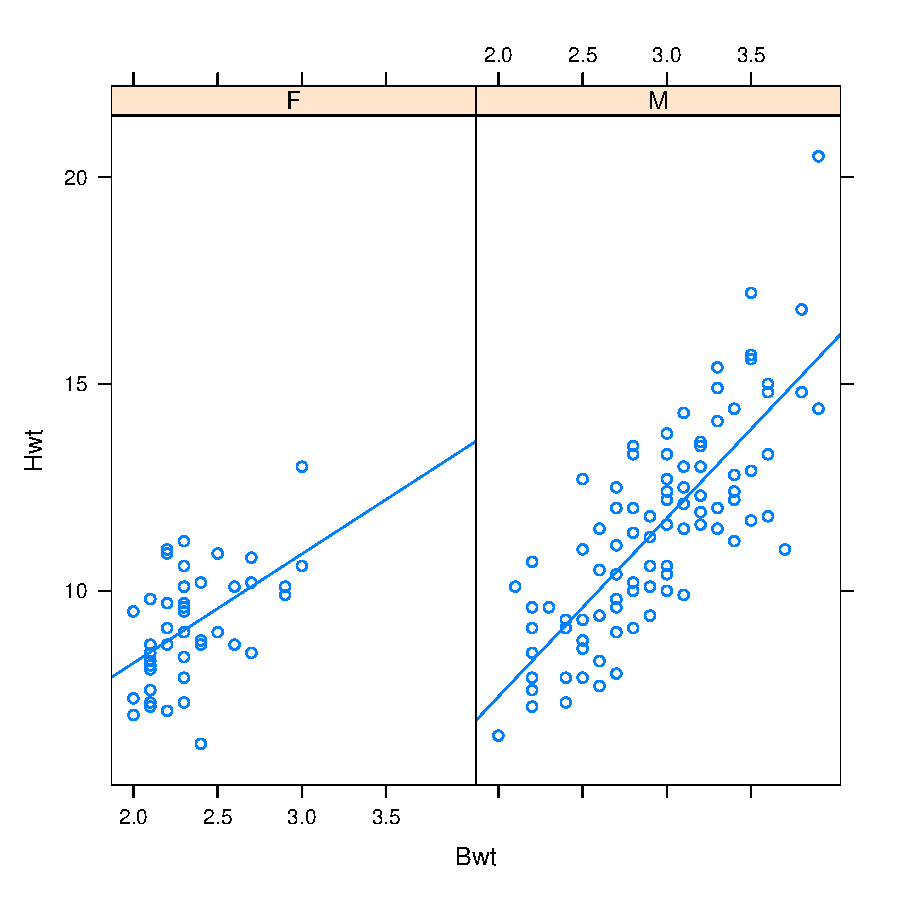
\includegraphics{figures/apps-figure}

  \caption{\small The cats data from package MASS.}
  \label{fig:cats}
\end{figure}

 
\chapter{Sweave Code} % (fold)
\label{app:sweave_code}

% app sweave_code (end)
\label{app:sweave-code}
Figure \ref{fig:code} shows the code used to produce the data analysis in Appendix \ref{sec:an_sweave_example} .

\begin{figure}
\begin{lstlisting}[style=sweave-top]

\end{lstlisting} 
\begin{lstlisting}[language={[latex]tex},numbers=none,style=sweave-tex]   
\section{Appendix: An Sweave Example}
\label{sec:append-sweave-exampl}
\end{lstlisting}
\begin{lstlisting}[language=R,numbers=none,style=sweave-r] 
<<prelim, echo=false,results=hide>>=
# load required libraries and set some options.
options(device="pdf")
library(lattice)
library(xtable)
data(cats, package="MASS")
@ 
\end{lstlisting}
%% note the use of escapechar and the \HL / \HLoff commands (defined in
%% listings-sweave.sty), to allow me to highlight \Sexpr expressions inline. 
\begin{lstlisting}[language={[latex]tex},numbers=none,style=sweave-tex] 
Consider the \texttt{cats} regression example from 
\citet{venables02:_moder_applied_statis_s_plus}. The data contains measurements 
of heart and body weight of #\HL#\Sexpr{nrow(cats)}#\HLoff# cats (\Sexpr{sum(cats$Sex=="F")}
female, #\HL#\Sexpr{sum(cats$Sex=="M")}#\HLoff# male). A linear regression
model of heart weight by bodyweight and sex can be fitted in R using the command
\end{lstlisting} 
\begin{lstlisting}[language=R,numbers=none,style=sweave-r] 
<<ols.model>>=
# OLS regression model 
lm1 <- lm(Hwt~Bwt*Sex, data=cats)
@ 
\end{lstlisting}
\begin{lstlisting}[language={[latex]tex},numbers=none,style=sweave-tex] 
Tests for significance of the coefficients are shown in Table~\ref{tab:coef}, a 
scatter plot including the regression lines is shown in Figure~\ref{fig:cats}.
\end{lstlisting}

\begin{lstlisting}[language=R,numbers=none,style=sweave-r] 
<<summary.table,results=tex,echo=FALSE>>=
# make a table summarizing the results
xtable(lm1, caption="Linear regression model for cats data.", 
       label="tab:coef")
@ 
\end{lstlisting}
\begin{lstlisting}[language={[latex]tex},numbers=none,style=sweave-tex] 
In this example, the code chunks that produce Table \ref{tab:coef} 
and Figure \ref{fig:cats} are replaced by their output when the 
final document is produced. 

\begin{figure}
  \centering
\end{lstlisting}
\begin{lstlisting}[language=R,numbers=none,style=sweave-r] 
<<ols.figure,fig=TRUE,echo=FALSE>>=
   # produce a plot of the regression lines by sex
   print(xyplot(Hwt~Bwt|Sex, data=cats,type=c("p","r")))
@ %def 
\end{lstlisting}
\begin{lstlisting}[language={[latex]tex},numbers=none,style=sweave-tex] 
  \caption{The cats data from package MASS.}
  \label{fig:cats}
\end{figure}
 
The code used to produce the data analysis shown here is presented in Figure 
\ref{fig:code}.
\end{lstlisting}
\begin{lstlisting}[style=sweave-bottom]

\end{lstlisting}
  \caption{The Sweave code used to produce Appendix I. The text is a mixture of
    LaTeX markup and chunks of R code (shown here in blocks with yellow
    background). The R code is replaced by its output when processed, resulting
    in a LaTeX document.}
\label{fig:code}
\end{figure}
 
%\backmatter

\bibliography{organsecon,data}

\end{document}
